% Options for packages loaded elsewhere
\PassOptionsToPackage{unicode}{hyperref}
\PassOptionsToPackage{hyphens}{url}
\PassOptionsToPackage{dvipsnames,svgnames,x11names}{xcolor}
%
\documentclass[
  12pt,
  a4paper,
]{scrreprt}

\usepackage{amsmath,amssymb}
\usepackage{iftex}
\ifPDFTeX
  \usepackage[T1]{fontenc}
  \usepackage[utf8]{inputenc}
  \usepackage{textcomp} % provide euro and other symbols
\else % if luatex or xetex
  \usepackage{unicode-math}
  \defaultfontfeatures{Scale=MatchLowercase}
  \defaultfontfeatures[\rmfamily]{Ligatures=TeX,Scale=1}
\fi
\usepackage{lmodern}
\ifPDFTeX\else  
    % xetex/luatex font selection
\fi
% Use upquote if available, for straight quotes in verbatim environments
\IfFileExists{upquote.sty}{\usepackage{upquote}}{}
\IfFileExists{microtype.sty}{% use microtype if available
  \usepackage[]{microtype}
  \UseMicrotypeSet[protrusion]{basicmath} % disable protrusion for tt fonts
}{}
\usepackage{xcolor}
\usepackage[left=3cm,,right=2cm,,top=3cm,,bottom=2cm]{geometry}
\setlength{\emergencystretch}{3em} % prevent overfull lines
\setcounter{secnumdepth}{5}


\providecommand{\tightlist}{%
  \setlength{\itemsep}{0pt}\setlength{\parskip}{0pt}}\usepackage{longtable,booktabs,array}
\usepackage{calc} % for calculating minipage widths
% Correct order of tables after \paragraph or \subparagraph
\usepackage{etoolbox}
\makeatletter
\patchcmd\longtable{\par}{\if@noskipsec\mbox{}\fi\par}{}{}
\makeatother
% Allow footnotes in longtable head/foot
\IfFileExists{footnotehyper.sty}{\usepackage{footnotehyper}}{\usepackage{footnote}}
\makesavenoteenv{longtable}
\usepackage{graphicx}
\makeatletter
\newsavebox\pandoc@box
\newcommand*\pandocbounded[1]{% scales image to fit in text height/width
  \sbox\pandoc@box{#1}%
  \Gscale@div\@tempa{\textheight}{\dimexpr\ht\pandoc@box+\dp\pandoc@box\relax}%
  \Gscale@div\@tempb{\linewidth}{\wd\pandoc@box}%
  \ifdim\@tempb\p@<\@tempa\p@\let\@tempa\@tempb\fi% select the smaller of both
  \ifdim\@tempa\p@<\p@\scalebox{\@tempa}{\usebox\pandoc@box}%
  \else\usebox{\pandoc@box}%
  \fi%
}
% Set default figure placement to htbp
\def\fps@figure{htbp}
\makeatother
% definitions for citeproc citations
\NewDocumentCommand\citeproctext{}{}
\NewDocumentCommand\citeproc{mm}{%
  \begingroup\def\citeproctext{#2}\cite{#1}\endgroup}
\makeatletter
 % allow citations to break across lines
 \let\@cite@ofmt\@firstofone
 % avoid brackets around text for \cite:
 \def\@biblabel#1{}
 \def\@cite#1#2{{#1\if@tempswa , #2\fi}}
\makeatother
\newlength{\cslhangindent}
\setlength{\cslhangindent}{1.5em}
\newlength{\csllabelwidth}
\setlength{\csllabelwidth}{3em}
\newenvironment{CSLReferences}[2] % #1 hanging-indent, #2 entry-spacing
 {\begin{list}{}{%
  \setlength{\itemindent}{0pt}
  \setlength{\leftmargin}{0pt}
  \setlength{\parsep}{0pt}
  % turn on hanging indent if param 1 is 1
  \ifodd #1
   \setlength{\leftmargin}{\cslhangindent}
   \setlength{\itemindent}{-1\cslhangindent}
  \fi
  % set entry spacing
  \setlength{\itemsep}{#2\baselineskip}}}
 {\end{list}}
\usepackage{calc}
\newcommand{\CSLBlock}[1]{\hfill\break\parbox[t]{\linewidth}{\strut\ignorespaces#1\strut}}
\newcommand{\CSLLeftMargin}[1]{\parbox[t]{\csllabelwidth}{\strut#1\strut}}
\newcommand{\CSLRightInline}[1]{\parbox[t]{\linewidth - \csllabelwidth}{\strut#1\strut}}
\newcommand{\CSLIndent}[1]{\hspace{\cslhangindent}#1}

\usepackage{dirtree}
\usepackage{amsmath}
\usepackage[explicit]{titlesec}
\usepackage{setspace}
\usepackage{caption}
\usepackage[hang,flushmargin]{footmisc}
\usepackage{etoolbox}
\usepackage[shortlabels]{enumitem}
\usepackage{booktabs}
\usepackage{ragged2e}
\usepackage{pdflscape}
\usepackage{fancyhdr}

\newcommand{\blandscape}{\begin{landscape}}
\newcommand{\elandscape}{\end{landscape}}
\renewcommand{\footnotesize}{\scriptsize}
\renewcommand{\footnoterule}{\noindent\rule{5cm}{0.4pt}\vspace{0.2cm}}
\setlength{\footnotesep}{0.5em}

\setlength{\parskip}{0.0em}
\AtBeginEnvironment{quote}{\setstretch{1.0}}

\titleformat{\section}{\normalfont\large\bfseries}{}{0pt}{\thesection\quad#1}[]
\titleformat{\subsection}{\normalfont\normalsize\bfseries}{}{0pt}{\thesubsection\quad#1}[]
\titleformat{\subsubsection}{\normalfont\normalsize\itshape}{}{0pt}{#1}[]
\titleformat{\paragraph}[runin]{\normalfont\normalsize\bfseries}{}{0pt}{#1}[]
\titleformat{\subparagraph}[runin]{\normalfont\normalsize\itshape}{}{0pt}{#1}[]

\titlespacing*{\section}{0pt}{20pt}{10pt}
\titlespacing*{\subsection}{0pt}{15pt}{10pt}
\titlespacing*{\subsubsection}{0pt}{10pt}{10pt}
\titlespacing*{\paragraph}{0pt}{10pt}{10pt}
\titlespacing*{\subparagraph}{0pt}{10pt}{10pt}
\makeatletter
\@ifpackageloaded{caption}{}{\usepackage{caption}}
\AtBeginDocument{%
\ifdefined\contentsname
  \renewcommand*\contentsname{Índice}
\else
  \newcommand\contentsname{Índice}
\fi
\ifdefined\listfigurename
  \renewcommand*\listfigurename{Lista de Figuras}
\else
  \newcommand\listfigurename{Lista de Figuras}
\fi
\ifdefined\listtablename
  \renewcommand*\listtablename{Lista de Tabelas}
\else
  \newcommand\listtablename{Lista de Tabelas}
\fi
\ifdefined\figurename
  \renewcommand*\figurename{Figura}
\else
  \newcommand\figurename{Figura}
\fi
\ifdefined\tablename
  \renewcommand*\tablename{Tabela}
\else
  \newcommand\tablename{Tabela}
\fi
}
\@ifpackageloaded{float}{}{\usepackage{float}}
\floatstyle{ruled}
\@ifundefined{c@chapter}{\newfloat{codelisting}{h}{lop}}{\newfloat{codelisting}{h}{lop}[chapter]}
\floatname{codelisting}{Listagem}
\newcommand*\listoflistings{\listof{codelisting}{Lista de Listagens}}
\makeatother
\makeatletter
\makeatother
\makeatletter
\@ifpackageloaded{caption}{}{\usepackage{caption}}
\@ifpackageloaded{subcaption}{}{\usepackage{subcaption}}
\makeatother
\makeatletter
\@ifpackageloaded{tcolorbox}{}{\usepackage[skins,breakable]{tcolorbox}}
\makeatother
\makeatletter
\@ifundefined{shadecolor}{\definecolor{shadecolor}{rgb}{.97, .97, .97}}{}
\makeatother
\makeatletter
\@ifundefined{codebgcolor}{\definecolor{codebgcolor}{HTML}{F0F2F4}}{}
\makeatother
\makeatletter
\ifdefined\Shaded\renewenvironment{Shaded}{\begin{tcolorbox}[sharp corners, boxrule=0pt, breakable, frame hidden, colback={codebgcolor}, enhanced]}{\end{tcolorbox}}\fi
\makeatother

\ifLuaTeX
\usepackage[bidi=basic]{babel}
\else
\usepackage[bidi=default]{babel}
\fi
\babelprovide[main,import]{brazilian}
% get rid of language-specific shorthands (see #6817):
\let\LanguageShortHands\languageshorthands
\def\languageshorthands#1{}
\usepackage{bookmark}

\IfFileExists{xurl.sty}{\usepackage{xurl}}{} % add URL line breaks if available
\urlstyle{same} % disable monospaced font for URLs
\hypersetup{
  pdftitle={Primeiro relatório da disciplina de demografia II - Roraima},
  pdfauthor={Gabriel de Jesus Pereira},
  pdflang={pt-br},
  colorlinks=true,
  linkcolor={blue},
  filecolor={Maroon},
  citecolor={Blue},
  urlcolor={Blue},
  pdfcreator={LaTeX via pandoc}}


\title{Primeiro relatório da disciplina de demografia II - Roraima}
\author{Gabriel de Jesus Pereira}
\date{março, 2025}

\begin{document}
\cleardoublepage
\thispagestyle{empty}
{\centering
\noindent\rule{\textwidth}{0.5pt}

\vspace{2ex}

{\Large\bfseries Universidade Federal da Paraíba \par}
\vspace{1ex}
{\Large\bfseries Centro de Ciências Exatas e da Natureza \par}
\vspace{1ex}
{\Large\bfseries Departamento de Estatística \par}

\vfill

{\large\bfseries Primeiro relatório da disciplina de demografia II -
Roraima \par}

\vfill

{\large Gabriel de Jesus Pereira \par}
\vfill
{\normalsize março, 2025 \par}


\noindent\rule{\textwidth}{0.5pt}

}
\renewcommand*\contentsname{\centering Sumário \thispagestyle{empty}}
{
\hypersetup{linkcolor=}
\setcounter{tocdepth}{2}
\tableofcontents
}

\pagenumbering{arabic}
\pagestyle{fancy}

\fancyhf{}
\fancyhead[RO, LE]{\thepage}
\fancyhead[LO]{\leftmark}
\fancyhead[RE]{\thepage}

\fancypagestyle{plain}{
  \pagestyle{fancy}
  \fancyhf{}
  \fancyhead[RO, LE]{\thepage}
  \fancyhead[RE]{\thepage}
  \renewcommand{\headrulewidth}{0pt}
}

\chapter{Introdução}\label{introduuxe7uxe3o}

Roraima é o estado menos populoso do Brasil, localizado na região Norte
e caracterizado por uma extensa área territorial, baixa densidade
demográfica e significativa presença de populações indígenas. Sua
dinâmica demográfica é influenciada por fatores como migração,
crescimento populacional e acesso a serviços de saúde.

\vspace{12pt}

Neste estudo, será realizada uma análise da cobertura de nascidos vivos
e de óbitos no estado, utilizando diferentes técnicas demográficas.
Algumas das abordagens baseiam-se na equação básica do crescimento
populacional e na taxa de fecundidade, além da aplicação dos métodos de
Brass, Hill e Leadermann para redistribuição de óbitos mal definidos.
Essas técnicas permitem avaliar a qualidade dos registros vitais e
fornecer estimativas mais precisas sobre a dinâmica populacional de
Roraima.

\chapter{Metodologia}\label{metodologia}

\section{Obtenção dos dados}\label{obtenuxe7uxe3o-dos-dados}

~~~Os dados demográficos utilizados neste estudo foram obtidos de duas
fontes principais. As informações sobre a população por faixa etária
foram extraídas do TABNET, uma ferramenta desenvolvida pelo DATASUS. O
TABNET é um tabulador genérico de domínio público que facilita a
organização e consulta rápida de dados conforme os critérios definidos,
enquanto o DATASUS fornece informações essenciais para a análise da
saúde pública e variáveis demográficas, contribuindo para a formulação
de políticas e programas de saúde. Alguns dos dados também foram obtidos
a partir do sistema Sidra, como é o caso dos dados populacionais e de
óbitos por faixa etária.

\section{Recursos computacionais}\label{recursos-computacionais}

~~~As análises apresentadas neste estudo foram realizadas utilizando a
linguagem de programação Python (VAN ROSSUM; DRAKE JR, 1995), com o
auxílio da biblioteca Pandas (TEAM, 2020) para manipulação de dados e da
biblioteca Matplotlib para visualização gráfica (HUNTER, 2007). Os
documentos do relatório foram elaborados com o Quarto (ALLAIRE;
DERVIEUX, 2024), um sistema de escrita e publicação científica. Todo o
código-fonte utilizado nas análises está disponível no GitHub.

\section{Métodos para estimação da cobertura de nascidos
vivos}\label{muxe9todos-para-estimauxe7uxe3o-da-cobertura-de-nascidos-vivos}

~~~A estimação do número de nascidos vivos é essencial para a análise
demográfica e epidemiológica, especialmente em contextos onde há
subnotificação ou inconsistências nos registros civis. Diversos métodos
podem ser utilizados para avaliar a cobertura dos nascimentos, como
comparações entre fontes de dados, modelagem estatística e ajustes
baseados em fatores demográficos. Nesta seção, serão apresentadas as
principais técnicas utilizadas para essa estimação.

\subsection{Razão de sexo dos nascimentos
(RSN)}\label{razuxe3o-de-sexo-dos-nascimentos-rsn}

~~~A Razão de Sexo dos Nascimentos (RSN) é um indicador que expressa a
relação entre o número de nascidos vivos do sexo masculino e feminino em
uma população. Geralmente, espera-se que essa razão esteja em torno de
105, indicando um leve predomínio de nascimentos masculinos sobre os
femininos.

\vspace{12pt}

O cálculo da RSN é feito pela seguinte fórmula:

\[
RSN = \frac{N_M}{N_F} \times 100 \text{,}
\] em que \(N_M\) representa o número de nascidos vivos do sexo
masculino e \(N_F\) do sexo feminino.

\vspace{12pt}

Valores significativamente diferentes do esperado podem indicar
problemas na qualidade dos dados, como erros de registro ou
subnotificação diferenciada por sexo.

\vspace{12pt}

Os limites do intervalo de confiança a \(95\%\) podem ser calculados a
partir da seguinte expressão:

\[
\left[x, y\right] = p_{M} \pm 1,96 \sqrt{\frac{p_{M}p_{F}}{n}} \text{,}
\] em que \(n\) é o número total de nascimentos, \(p_{M}\) é a proporção
de nascidos vivos do sexo masculino e \(p_{F}\) do sexo feminino.

\vspace{12pt}

Por fim, para verificar se a qualidade de registro de nascimentos é boa,
basta verificar se o resultado das relações de sexo está incluso no
intervalo \(\left[a, b\right]\):

\[
a = \frac{x}{1 - x} \times 100 \text{ e } b = \frac{y}{1-y}\times 100\text{.}
\]

\vspace{12pt}

Esse método foi utilizado apenas para os anos de 2010 e 2020, com dados
obtidos do SINASC.

\subsection{Método que utiliza a equação básica do crescimento
populacional}\label{muxe9todo-que-utiliza-a-equauxe7uxe3o-buxe1sica-do-crescimento-populacional}

O método que utiliza a equação básica do crescimento populacional é
bastante simples, principalmente por assumir que a popuação é fechada.
Dessa forma, a estimativa de nascidos vivos será expresso pela equação:

\[
N_t = P_n - P_{0} + O_t
\] em que \(P_n\) são os nascidos vivos no instante \(n\), P\_\{0\} no
instante inicial e \(O_t\) os óbitos no período de estudo.

\vspace{12pt}

A partir dessa expressão, estima-se a cobertura dos nascimentos da
seguinte forma:

\[
\text{Cobertura dos nascimentos} = \frac{\text{Nascimentos registrados}\left(t\right)}{\text{Nascimentos esperados}\left(t\right)} \times 100
\]

\vspace{12pt}

Para esse método foi considerado os dados obtidos fornecidos pelo SIM e
pelo Registro Civil, para anos entre 2010 e 2020.

\subsection{Método que faz uso das taxas de
fecundidade}\label{muxe9todo-que-faz-uso-das-taxas-de-fecundidade}

Neste método serão utilizadas as taxas de fecundidade do estado de
Roraima. Para estimar a cobertura nesse método, será utilizada a
seguinte expressão:

\[
C_i = \frac{NV_{obs}\left(i\right)}{NV_{est}\left(i\right)} \text{,}
\] em que \(NV_{obs}\left(i\right)\) é o total de nascidos vivos
observados na região \(i\) e \(NV_{est}\left(i\right)\) é o total de
nascidos vivos estimados na região \(i\).

\vspace{12pt}

Para encontrar a estimativa dos nascidos vivos
\(NV_{est}\left(i\right)\), será utilizado a taxa de fecundidade do
estado de Roraima, que pode ser encontrado a partir da seguinte
expressão:

\[
NV_{est} = \sum^{49}_{j=15} TEF_{j}\left(i\right) \times TM_{j} \text{,}
\] em que \(TEF_{j}\left(i\right)\) é a taxa específica de fecundidade
na faixa etária quinquenal \(j\) da região \(i\) e \(TM_j\) é o total de
mulheres na faixa etária quinquenal \(j\) da região \(j\).

\vspace{12pt}

Esse método foi aplicado apenas para os anos de 2000 e 2010, com dados
obtidos pelo TABNET.

\subsection{Método que faz uso da informação do SINASC e do
IBGE}\label{muxe9todo-que-faz-uso-da-informauxe7uxe3o-do-sinasc-e-do-ibge}

Aqui são utilizadas as estimativas de nascidos vivos fornecidos pelo
IBGE e os nascidos vivos fornecidos pelo SINASC. Por fim, para estimar a
cobertura, basta calcular utilizar a seguinte expressão:

\[
C_i = \frac{NV_{obs}\left(i\right)}{NV_{est}\left(i\right)}
\]

\section{Métodos para estimação da cobertura de
óbito}\label{muxe9todos-para-estimauxe7uxe3o-da-cobertura-de-uxf3bito}

A cobertura dos óbitos refere-se à proporção de mortes registradas em
relação ao total de óbitos ocorridos em uma população. Em contextos onde
há subnotificação ou falhas nos sistemas de informação, diferentes
métodos são empregados para estimar a verdadeira magnitude da
mortalidade.

\vspace{12pt}

Entre as principais abordagens utilizadas, destacam-se os métodos
demográficos indiretos, como o método de Brass, que utiliza informações
da estrutura etária da população e da mortalidade infantil para estimar
a cobertura. Além disso, comparações entre diferentes bases de dados,
modelagem estatística e técnicas de reconciliação de fontes são
amplamente empregadas para corrigir deficiências nos registros.

\vspace{12pt}

Esses métodos são fundamentais para garantir a confiabilidade dos
indicadores de mortalidade e subsidiar políticas públicas voltadas à
saúde e ao planejamento populacional. Além disso, esse método foi
aplicado apenas para os anos de 2010 e 2020.

\subsection{Método que faz uso da equação básica do crescimento
populacional}\label{muxe9todo-que-faz-uso-da-equauxe7uxe3o-buxe1sica-do-crescimento-populacional}

De forma semelhante ao método de cobertura de nascidos vivos que faz uso
da equação básica do crescimento populacional, para estimar os óbitos,
basta isolar a sua componente:

\[
O_t = N_t + P_{0} - P_n
\]

Por fim, para estimar a cobertura de óbitos, utiliza-se a seguinte
expressão:

\[
\text{Cobertura dos óbitos} = \frac{\text{Óbitos registrados}\left(t\right)}{\text{Óbitos esperados}\left(t\right)} \times 100
\]

\vspace{12pt}

A cobertura foi estimada apenas para o ano de 2010, utilizando-se de
dados do SINASC, SIM e do censo seu cálculo.

\subsection{Método da Equação do Balanço de Crescimento de
Brass}\label{muxe9todo-da-equauxe7uxe3o-do-balanuxe7o-de-crescimento-de-brass}

Esse método avalia a cobertura de óbitos da população a partir dos cinco
anos de idade. Para fazer sua aplicação, é necessário considerar a
população estável, a cobertura de óbitos é constante por idade a partir
dos 5 anos e as distribuições por idade da população não devem conter
erros de declaração.

\vspace{12pt}

Nesse método é utilizado uma regressão linear, a partir da qual será
estimada o fator de correção dos óbitos \(\left(k\right)\), a taxa de
crescimento da população estável \(\left(r\right)\). Dessa forma, essa
regressão linear terá a seguinte relação:

\[
\frac{N\left(a\right)}{N\left(a+\right)} = r + k\frac{D^{'}\left(a+\right)}{N\left(a+\right)}\text{,}
\] em que \(N\left(a\right)\) é a população exata na idade \(a\),
\(N\left(a+\right)\) o somatório de pessoas que estão na idade exata até
um limite de idades \(w\) qualquer e \(D^{'}\left(a+\right)\) são os
óbitos registrados e afetados por erros na idade \(a+\).

\vspace{12pt}

Após o ajuste da regressão linear, a cobertura dos óbitos será dada por:

\[
C = \frac{1}{k}\text{,}
\] em que se o fator de correção for \(k > 1\) implica em sub-registro e
\(k<1\) implica em sobre-registro.

\vspace{12pt}

O método de Brass foi considerado apenas para o ano de 2010 e 2020, para
cada um dos sexos.

\subsection{Método de Hill}\label{muxe9todo-de-hill}

~~~O método de Hill é uma abordagem utilizada para estimar a cobertura
de óbitos. Ele se baseia em três pressupostos: a cobertura de cada censo
é a mesma para todas as idades; a completude dos registros de óbitos é
uniforme para todas as idades acima de um limite mínimo; e a população é
fechada. Diferentemente de outros métodos, a estabilidade populacional
não é um requisito nesse caso.

\vspace{12pt}

Para seu cálculo, são necessários dados sobre o número de indivíduos,
organizados em grupos etários de cinco em cinco anos, incluindo o
intervalo aberto \(a+\) (com aa sendo a idade mais avançada possível),
em dois momentos no tempo (geralmente dois anos censitários). Além
disso, é necessário o número de óbitos ocorridos nessa população, também
agrupados em intervalos etários quinquenais e no intervalo aberto
\(a+\), durante o período intercensitário.

\vspace{12pt}

O primeiro passo é estimar as taxas de natalidade e de mortalidade
parciais e, para isso, é preciso acumular a população e o número de
mortes para as idades \(x\) em diante. Assim, no caso da população, a
seguinte equação é usada:

\[
N\left(x+\right) = \sum^{A-5}_{y=x} {_5}N_y + {_\infty}N_A
\] em que \(A\) é a idade no início do intervalo aberto.

\vspace{12pt}

O segundo passo é calcular o número de pessoas-anos vividos, que pode
ser calculado da seguinte forma:

\[
\text{PYL}\left(x+\right) = \left(t_{2} - t_{1}\right)\left(_{\infty}N_{x}\left(t_{1}\right)\times_{\infty}N_{x}\left(t_{2}\right)\right)^{1/2}
\] em que \(t_{1}\) é o ano do primeiro censo e \(t_{2}\) é o ano do
segundo censo.

\vspace{12pt}

No terceiro passo, deve-se calcular o número de pessoas que passaram
para a idade \(x\), que é estimada como a média geométrica dos números
em uma coorte em tempos \(t_{1}\) e \(t_{2}\) dividido por 5,
multiplicado pelo comprimento do período entre os censos, em anos,
usando a seguinte fórmula:

\[
N\left(x\right) = \frac{t}{5}\left(_{5}N_{x-5}\left(t_{1}\right)\times_{5}N_{x-5}\left(t_{2}\right)\right)^{1/2}
\]

\vspace{12pt}

Após o terceiro passo, deve-se calcular taxas parciais de natalidade,
mortalidade e crescimento, as quais podem ser calculadas a partir das
seguintes equações:

\[
b\left(x+\right) = \frac{N\left(x\right)}{PYL\left(x+\right)}
\]

\[
d\left(x+\right) = \frac{D\left(x+\right)}{PYL\left(x+\right)}
\]

\[
r\left(x+\right) = \frac{_{\infty}N_{x}\left(t_{2}\right) - _{\infty}N_{x}\left(t_{1}\right)}{PYL\left(x+\right)}\text{, }
\]

Por último, basta ajustar uma regressão linear, utilizando
\(d\left(x+\right)\) como variável independente e \(r\left(x+\right)\)
como variável dependente. Após o ajuste, será estimado o intercepto
\(a\) e o coeficiente \(b\), que serão utilizados para estimar um valor
\(k_{1}\) e \(k_{2}\) e da cobertura final. Para estimar a cobertura,
deve-se verificar se
\(k_{1}/k_{2} = e^{a\left(t_{2} - t_{1}\right)} < 1\). Caso essa
condição seja satisfeita, assume-se que \(k_{2}\) é igual a 1 e a
cobertura estimada será \(c = e^{a\left(t_{2} - t_{1}\right)} / b\).
Caso contrário, a cobertura estimada será
\(c = e^{-a\left(t_{2} - t_{1}\right)} / b\).

\vspace{12pt}

Esse método foi aplicado utilizando os dados do censo de 2010 e 2022,
para o estado de Roraima. No caso dos óbitos, foram utilizados os dados
disponibilizados pelo SIM.

\vspace{12pt}

O método de Hill foi utilizado utilizando-se de dados do censo de 2010 e
2022 e dados fornecidos pelo Registro Civil.

\subsection{Método de Leadermann para
redistribuição}\label{muxe9todo-de-leadermann-para-redistribuiuxe7uxe3o}

~~~O método de Leadermann é uma abordagem utilizada para redistribuir
óbitos classificados com causas mal definidas entre categorias
específicas de mortalidade. Essa técnica busca minimizar o impacto da
subnotificação e da imprecisão nos registros, permitindo uma estimativa
mais fiel da estrutura de mortalidade de uma população.

\vspace{12pt}

A redistribuição é feita com base na suposição de que a proporção de
óbitos por causas definidas segue um padrão semelhante ao dos óbitos mal
definidosa. Assim, os óbitos mal classificados são redistribuídos
proporcionalmente entre as categorias bem definidas, considerando a
estrutura observada nos registros mais completos. Isso é feito
utilizando-se uma regressão linear

\vspace{12pt}

A equação de redistribuição dos óbitos por causas mal definidas para uma
determinada área é dada por:

\[
O_j = Y_j - X \beta_{j}
\] em que \(O_j\) são os óbitos redistribuídos da causa \(j\), \(Y_j\)
os óbitos observados da causa \(j\), \(\beta_j\) é o fator de
redistribuição da causa \(j\) e \(X\) são os óbitos da causa mal
definida.

\vspace{12pt}

O método de Leadermann foi utilizado apenas para o ano de 2022.

\chapter{Resultado}\label{resultado}

\section{Resultado da estimação de cobertura de
nascimentos}\label{resultado-da-estimauxe7uxe3o-de-cobertura-de-nascimentos}

Nesta seção serão apresentadas cada uma das técnicas utilizadas para
analisar e estimar a cobertura dos nascidos vivos. O primeiro deles será
o RSN, depois o método de estimação utilizando a equação do crescimento
populacional, o que o utiliza as taxas de fecundidade e por último o que
utiliza as estimativas do IBGE e os dados do SINASC.

\subsection{Razão de Sexo dos Nascimentos
(RSN)}\label{razuxe3o-de-sexo-dos-nascimentos-rsn-1}

A abaixo apresenta os valores da Razão de Sexo dos Nascimentos (RSN)
para os anos de 2010 e 2020. Esse indicador expressa a relação entre os
nascidos vivos do sexo masculino e feminino, sendo esperado um valor em
torno de 105 em condições normais.

\begin{longtable}[]{@{}lllllllll@{}}
\caption{Resultados da Razão de sexo dos nascimentos para o ano de 2010
e 2020}\label{T_c7532}\tabularnewline
\toprule\noalign{}
Ano & Masculino & Feminino & RSN & total & x & y & a & b \\
\midrule\noalign{}
\endfirsthead
\toprule\noalign{}
Ano & Masculino & Feminino & RSN & total & x & y & a & b \\
\midrule\noalign{}
\endhead
\bottomrule\noalign{}
\endlastfoot
2010 & 4990 & 4748 & 105,097 & 9738 & 0,507 & 0,518 & 102,974 &
107,265 \\
2020 & 7075 & 6684 & 105,850 & 13759 & 0,510 & 0,519 & 104,044 &
107,688 \\
\end{longtable}

Em 2010, a RSN foi de 105,097, indicando que para cada 100 meninas
nasceram aproximadamente 105 meninos. Já em 2020, esse valor aumentou
para 105,850, sugerindo um leve crescimento na proporção de nascimentos
masculinos em relação aos femininos. Além disso, ao observar o intervalo
\(\left[a, b\right]\), tem-se que há uma boa qualidade no registro dos
dados, pois os valores estimados da \(RSN\) estão contidos dentro do
intervalo.

\subsection{Método que utiliza a equação básica do crescimento
populacional}\label{muxe9todo-que-utiliza-a-equauxe7uxe3o-buxe1sica-do-crescimento-populacional-1}

~~~Para o método que utiliza a equação básica do crescimento
populacional, foi estimado um nascimento esperado de 137299, bastante
próximo ao valor observado no período de
\(N_{\text{observado}} = 128467\). Além disso, o óbito total estimado no
período foi de \(O_t = 24778\).

\begin{longtable}[]{@{}lllll@{}}
\caption{}\label{T_dc1fd}\tabularnewline
\toprule\noalign{}
Ano & Óbito & População & nascimento\_esperado & C \\
\midrule\noalign{}
\endfirsthead
\toprule\noalign{}
Ano & Óbito & População & nascimento\_esperado & C \\
\midrule\noalign{}
\endhead
\bottomrule\noalign{}
\endlastfoot
2020 & 3580 & 563000 & 137299 & 93,567 \\
2010 & 1640 & 450479 & 137299 & 93,567 \\
\end{longtable}

Por fim, a estimativa final da cobertura foi de 93,567\%, o que indica
um valor de cobertura bastante alto pelo método que utiliza a equação do
crescimento populacional.

\blandscape

\subsection{Método que faz uso das taxas de
fecundidade}\label{muxe9todo-que-faz-uso-das-taxas-de-fecundidade-1}

~~~Comparado ao método que utiliza a equação básica do crescimento
populacional, o que faz uso das taxas de fecundidade entrega respostas
bem melhores. Por exemplo, o número de nascidos vivos estimados de 2000
foi de 10897,410 e o de 2010 foi de 11088,013, bastante próximo de seus
valores observados (9744 e 9738, respectivamente).

\begin{longtable}[]{@{}lllllllll@{}}
\caption{}\label{T_31a78}\tabularnewline
\toprule\noalign{}
Faixa etária & Mulheres\_2000 & Mulheres\_2010 & TFE\_2000 & TFE\_2010 &
NV\_2000 & NV\_2010 & C\_2000 & C\_2010 \\
\midrule\noalign{}
\endfirsthead
\toprule\noalign{}
Faixa etária & Mulheres\_2000 & Mulheres\_2010 & TFE\_2000 & TFE\_2010 &
NV\_2000 & NV\_2010 & C\_2000 & C\_2010 \\
\midrule\noalign{}
\endhead
\bottomrule\noalign{}
\endlastfoot
15 a 19 anos & 20760 & 25260 & 0,159 & 0,111 & 10897,410 & 11088,013 &
0,894 & 0,878 \\
20 a 24 anos & 16294 & 21788 & 0,214 & 0,150 & 10897,410 & 11088,013 &
0,894 & 0,878 \\
25 a 29 anos & 13430 & 21792 & 0,167 & 0,121 & 10897,410 & 11088,013 &
0,894 & 0,878 \\
30 a 34 anos & 11606 & 18669 & 0,100 & 0,081 & 10897,410 & 11088,013 &
0,894 & 0,878 \\
35 a 39 anos & 10175 & 14839 & 0,055 & 0,045 & 10897,410 & 11088,013 &
0,894 & 0,878 \\
40 a 44 anos & 7926 & 12269 & 0,018 & 0,015 & 10897,410 & 11088,013 &
0,894 & 0,878 \\
45 a 49 anos & 5710 & 10379 & 0,002 & 0,002 & 10897,410 & 11088,013 &
0,894 & 0,878 \\
\end{longtable}

Com o resultado da cobertura estimada, tem-se uma cobertura de 89,4\% no
ano de 2000 e de 87,8\% no ano de 2010, o que indica de fato uma boa
cobertura de nascidos vivos, utilizando o método de estimação que faz
uso das taxas de fecundidade.

\elandscape

\subsection{Método que faz uso dos dados do IBGE e
SINASC}\label{muxe9todo-que-faz-uso-dos-dados-do-ibge-e-sinasc}

Por último, o método que utiliza os nascidos vivos estimados do IBGE e
dos valores observados de nascidos vivos do SINASC, foi o que apresentou
os melhores resultados para estimação da cobertura de nascidos vivos.

\begin{longtable}[]{@{}llll@{}}
\caption{}\label{T_2fa52}\tabularnewline
\toprule\noalign{}
Ano & IBGE & SINASC & Cobertura \\
\midrule\noalign{}
\endfirsthead
\toprule\noalign{}
Ano & IBGE & SINASC & Cobertura \\
\midrule\noalign{}
\endhead
\bottomrule\noalign{}
\endlastfoot
2020 & 13991 & 13760 & 0,983 \\
2010 & 10686 & 9738 & 0,911 \\
\end{longtable}

Para a cobertura de 2020, foi estimado um valor de 98,3\% para o ano de
2020 e de 91,1\% para o ano de 2010.

\section{Resultados da estimação de cobertura de
óbitos}\label{resultados-da-estimauxe7uxe3o-de-cobertura-de-uxf3bitos}

Agora serão apresentadas cada uma das técnicas utilizadas para analisar
e estimar a cobertura dos óbitos. O primeiro deles será o método que
utiliza a equação básica do crescimento populacional, depois o método de
Brass, o que utiliza o método de Hill e, por útlimo, o método de
Leadermann para redistribuição de óbitos mal definidos.

\subsection{Método que utiliza a equação básica do crescimento
populacional}\label{muxe9todo-que-utiliza-a-equauxe7uxe3o-buxe1sica-do-crescimento-populacional-2}

A cobertura estimada pelo método que utiliza a equação básica do
crescimento populacional não apresentou boas estimativas, tendo obtido
uma estimativa para a cobertura de -80,3534\%, indicando que o método
subestimou os óbitos, principalmente devido ao crescimento da população
obtido no ano de 2010. Para o seu cálculo, foi utilizado os nascidos
vivos totais no período de 2000 a 2010 (\(N_t = 106618\)) e os óbitos
totais observados no período (\(O_t = 15640\)).

\begin{longtable}[]{@{}llll@{}}
\caption{}\label{T_9d74d}\tabularnewline
\toprule\noalign{}
Ano & População & obito\_estimado & C \\
\midrule\noalign{}
\endfirsthead
\toprule\noalign{}
Ano & População & obito\_estimado & C \\
\midrule\noalign{}
\endhead
\bottomrule\noalign{}
\endlastfoot
2010 & 450479 & -19464 & -80,353473 \\
2000 & 324397 & -19464 & -80,353473 \\
\end{longtable}

\subsection{Método da equação do balanço de crescimento de
Brass}\label{muxe9todo-da-equauxe7uxe3o-do-balanuxe7o-de-crescimento-de-brass-1}

Pelo método de Brass e considerando os dois anos para cada sexo,
observa-se, pelo fator de correção \(k\), um sub-registro da cobertura
de óbitos, pois todos os fatores de correção estão acima de 1
\(\left(k > 1\right)\).

\begin{longtable}[]{@{}llllllll@{}}
\caption{Método de Brass para homens.}\label{T_dcd47}\tabularnewline
\toprule\noalign{}
Faixa etária & Óbitos & População & N(a) & N(a+) & D\textquotesingle(a+)
& y & x \\
\midrule\noalign{}
\endfirsthead
\toprule\noalign{}
Faixa etária & Óbitos & População & N(a) & N(a+) & D\textquotesingle(a+)
& y & x \\
\midrule\noalign{}
\endhead
\bottomrule\noalign{}
\endlastfoot
0 a 4 anos & 56 & 24319 & nan & 228859 & 1000 & nan & 0.004370 \\
5 a 9 anos & 6 & 25254 & 5060 & 204540 & 944 & 0.024738 & 0.004615 \\
10 a 14 anos & 8 & 26321 & 5556 & 179286 & 938 & 0.030990 & 0.005232 \\
15 a 19 anos & 40 & 23737 & 5179 & 152965 & 930 & 0.033857 & 0.006080 \\
20 a 24 anos & 57 & 21828 & 4286 & 129228 & 890 & 0.033166 & 0.006887 \\
25 a 29 anos & 53 & 21398 & 4576 & 107400 & 833 & 0.042607 & 0.007756 \\
30 a 34 anos & 70 & 18326 & 4282 & 86002 & 780 & 0.049790 & 0.009070 \\
35 a 39 anos & 51 & 14909 & 3362 & 67676 & 710 & 0.049678 & 0.010491 \\
40 a 44 anos & 48 & 13039 & 3097 & 52767 & 659 & 0.058692 & 0.012489 \\
45 a 49 anos & 58 & 11142 & 2568 & 39728 & 611 & 0.064640 & 0.015380 \\
50 a 54 anos & 73 & 8831 & 2099 & 28586 & 553 & 0.073428 & 0.019345 \\
55 a 59 anos & 75 & 6719 & 1486 & 19755 & 480 & 0.075221 & 0.024298 \\
60 a 64 anos & 64 & 4942 & 1289 & 13036 & 405 & 0.098880 & 0.031068 \\
65 a 69 anos & 62 & 3213 & 885 & 8094 & 341 & 0.109340 & 0.042130 \\
70 a 74 anos & 75 & 2200 & 628 & 4881 & 279 & 0.128662 & 0.057160 \\
75 a 79 anos & 55 & 1334 & 320 & 2681 & 204 & 0.119358 & 0.076091 \\
80 anos e mais & 149 & 1347 & nan & 1347 & 149 & nan & 0.110616 \\
0 a 4 anos & 112 & 32994 & nan & 320392 & 1869 & nan & 0.005833 \\
5 a 9 anos & 7 & 32530 & 6559 & 287398 & 1757 & 0.022822 & 0.006113 \\
10 a 14 anos & 12 & 29925 & 6140 & 254868 & 1750 & 0.024091 &
0.006866 \\
15 a 19 anos & 43 & 28873 & 5911 & 224943 & 1738 & 0.026278 &
0.007726 \\
20 a 24 anos & 77 & 29360 & 5892 & 196070 & 1695 & 0.030050 &
0.008645 \\
25 a 29 anos & 96 & 27568 & 5884 & 166710 & 1618 & 0.035295 &
0.009705 \\
30 a 34 anos & 73 & 24602 & 5614 & 139142 & 1522 & 0.040347 &
0.010938 \\
35 a 39 anos & 114 & 24419 & 5071 & 114540 & 1449 & 0.044273 &
0.012651 \\
40 a 44 anos & 98 & 21464 & 5154 & 90121 & 1335 & 0.057190 & 0.014813 \\
45 a 49 anos & 98 & 16924 & 3700 & 68657 & 1237 & 0.053891 & 0.018017 \\
50 a 54 anos & 102 & 14317 & 3372 & 51733 & 1139 & 0.065181 &
0.022017 \\
55 a 59 anos & 129 & 11850 & 2487 & 37416 & 1037 & 0.066469 &
0.027715 \\
60 a 64 anos & 171 & 9086 & 2150 & 25566 & 908 & 0.084096 & 0.035516 \\
65 a 69 anos & 158 & 6857 & 1662 & 16480 & 737 & 0.100850 & 0.044721 \\
70 a 74 anos & 168 & 4576 & 1189 & 9623 & 579 & 0.123558 & 0.060168 \\
75 a 79 anos & 139 & 2570 & 688 & 5047 & 411 & 0.136319 & 0.081435 \\
80 anos e mais & 272 & 2477 & nan & 2477 & 272 & nan & 0.109810 \\
\end{longtable}

\begin{longtable}[]{@{}llllllll@{}}
\caption{Método de Brass para mulheres.}\label{T_14dea}\tabularnewline
\toprule\noalign{}
Faixa etária & Óbitos & População & N(a) & N(a+) & D\textquotesingle(a+)
& y & x \\
\midrule\noalign{}
\endfirsthead
\toprule\noalign{}
Faixa etária & Óbitos & População & N(a) & N(a+) & D\textquotesingle(a+)
& y & x \\
\midrule\noalign{}
\endhead
\bottomrule\noalign{}
\endlastfoot
0 a 4 anos & 53 & 23284 & nan & 221620 & 576 & nan & 0.002599 \\
5 a 9 anos & 4 & 24113 & 4804 & 198336 & 523 & 0.024222 & 0.002637 \\
10 a 14 anos & 5 & 25590 & 5431 & 174223 & 519 & 0.031173 & 0.002979 \\
15 a 19 anos & 13 & 23250 & 5025 & 148633 & 514 & 0.033808 & 0.003458 \\
20 a 24 anos & 18 & 21788 & 4295 & 125383 & 501 & 0.034255 & 0.003996 \\
25 a 29 anos & 27 & 21792 & 4422 & 103595 & 483 & 0.042685 & 0.004662 \\
30 a 34 anos & 20 & 18669 & 4309 & 81803 & 456 & 0.052675 & 0.005574 \\
35 a 39 anos & 16 & 14839 & 3294 & 63134 & 436 & 0.052175 & 0.006906 \\
40 a 44 anos & 20 & 12269 & 2866 & 48295 & 420 & 0.059344 & 0.008697 \\
45 a 49 anos & 29 & 10379 & 2331 & 36026 & 400 & 0.064703 & 0.011103 \\
50 a 54 anos & 36 & 8087 & 1917 & 25647 & 371 & 0.074746 & 0.014466 \\
55 a 59 anos & 43 & 5928 & 1372 & 17560 & 335 & 0.078132 & 0.019077 \\
60 a 64 anos & 48 & 4131 & 1050 & 11632 & 292 & 0.090268 & 0.025103 \\
65 a 69 anos & 47 & 2793 & 735 & 7501 & 244 & 0.097987 & 0.032529 \\
70 a 74 anos & 42 & 1960 & 544 & 4708 & 197 & 0.115548 & 0.041844 \\
75 a 79 anos & 42 & 1241 & 310 & 2748 & 155 & 0.112809 & 0.056405 \\
80 anos e mais & 113 & 1507 & nan & 1507 & 113 & nan & 0.074983 \\
0 a 4 anos & 82 & 31758 & nan & 316315 & 1060 & nan & 0.003351 \\
5 a 9 anos & 4 & 30713 & 6225 & 284557 & 978 & 0.021876 & 0.003437 \\
10 a 14 anos & 18 & 28288 & 5818 & 253844 & 974 & 0.022920 & 0.003837 \\
15 a 19 anos & 18 & 28002 & 5473 & 225556 & 956 & 0.024264 & 0.004238 \\
20 a 24 anos & 29 & 29351 & 5831 & 197554 & 938 & 0.029516 & 0.004748 \\
25 a 29 anos & 27 & 28132 & 6083 & 168203 & 909 & 0.036165 & 0.005404 \\
30 a 34 anos & 30 & 25129 & 5688 & 140071 & 882 & 0.040608 & 0.006297 \\
35 a 39 anos & 46 & 24524 & 5163 & 114942 & 852 & 0.044918 & 0.007412 \\
40 a 44 anos & 43 & 22316 & 5341 & 90418 & 806 & 0.059070 & 0.008914 \\
45 a 49 anos & 44 & 17520 & 4003 & 68102 & 763 & 0.058779 & 0.011204 \\
50 a 54 anos & 66 & 14070 & 3187 & 50582 & 719 & 0.063007 & 0.014215 \\
55 a 59 anos & 72 & 11618 & 2512 & 36512 & 653 & 0.068799 & 0.017885 \\
60 a 64 anos & 69 & 8999 & 2067 & 24894 & 581 & 0.083032 & 0.023339 \\
65 a 69 anos & 87 & 6525 & 1576 & 15895 & 512 & 0.099151 & 0.032211 \\
70 a 74 anos & 76 & 4154 & 1029 & 9370 & 425 & 0.109819 & 0.045358 \\
75 a 79 anos & 101 & 2479 & 584 & 5216 & 349 & 0.111963 & 0.066910 \\
80 anos e mais & 248 & 2737 & nan & 2737 & 248 & nan & 0.090610 \\
\end{longtable}

\begin{longtable}[]{@{}llllll@{}}
\caption{}\label{T_a87cd}\tabularnewline
\toprule\noalign{}
Ano & Sexo & k & r & R² & C = 1/k \\
\midrule\noalign{}
\endfirsthead
\toprule\noalign{}
Ano & Sexo & k & r & R² & C = 1/k \\
\midrule\noalign{}
\endhead
\bottomrule\noalign{}
\endlastfoot
2010 & homens & 1,474515 & 0,033951 & 0,862382 & 0,678189 \\
2010 & mulheres & 1,702502 & 0,037126 & 0,868452 & 0,587371 \\
2022 & homens & 1,582704 & 0,021985 & 0,954212 & 0,631830 \\
2022 & mulheres & 1,542196 & 0,032000 & 0,825744 & 0,648426 \\
\end{longtable}

Além disso, a maioria das coberturas estimadas ficaram próximas de 60\%,
o que indica, pelo método de Brass, uma cobertura deficiente, para os
dois sexos. Embora isso tenha sido um padrão para os dois sexos e anos
considerados, o ano de 2010, considerando o sexo masculino, foi o que
apresentou a maior cobertura, próximo de 68\%.

\blandscape

\subsection{Método de Hill}\label{muxe9todo-de-hill-1}

~~~Aplicando o método de Hill para o sexo masculino e utilizando
regressão para a estimação dos coeficientes e do intercepto no período
intercensitário, obteve-se um intercepto de valor \(-0,06346829\)
\(\left(a = -0,06346829\right)\) e um coeficiente \(b = 1,78109927\).
Além disso, como
\(\frac{k_{1}}{k_{2}} = e^{a\left(t_{2} - t_{1}\right)} = 0,46690964 < 1\),
assumiu-se \(k_{2} = 1\), resultando em \(k_{1} = 0,46690964\). Dessa
forma, a estimativa final para a cobertura de óbitos do sexo masculino
foi de apenas \(26,2146\%\).

\begin{longtable}[]{@{}lllllllllllll@{}}
\caption{Método de Hill para o sexo
masculino.}\label{T_23de2}\tabularnewline
\toprule\noalign{}
Faixa etária & 5Dx & 5N(t1) & N1(x+) & D(x+) & 5N(t2) & N2(x+) & PYL &
N(X) & b(x+) & d(x+) & r(x+) & b(x+) - r(x+) \\
\midrule\noalign{}
\endfirsthead
\toprule\noalign{}
Faixa etária & 5Dx & 5N(t1) & N1(x+) & D(x+) & 5N(t2) & N2(x+) & PYL &
N(X) & b(x+) & d(x+) & r(x+) & b(x+) - r(x+) \\
\midrule\noalign{}
\endhead
\bottomrule\noalign{}
\endlastfoot
0 a 4 anos & 168 & 24319 & 228859 & 2869 & 32994 & 320392 & 3249421,695
& nan & nan & nan & nan & nan \\
5 a 9 anos & 13 & 25254 & 204540 & 2701 & 32530 & 287398 & 2909459,008 &
67503,475 & 0,023 & 0,001 & 0,028 & -0,005 \\
10 a 14 anos & 20 & 26321 & 179286 & 2688 & 29925 & 254868 & 2565146,010
& 65977,128 & 0,026 & 0,001 & 0,029 & -0,004 \\
15 a 19 anos & 83 & 23737 & 152965 & 2668 & 28873 & 224943 & 2225940,355
& 66161,964 & 0,030 & 0,001 & 0,032 & -0,003 \\
20 a 24 anos & 134 & 21828 & 129228 & 2585 & 29360 & 196070 &
1910139,704 & 63358,105 & 0,033 & 0,001 & 0,035 & -0,002 \\
25 a 29 anos & 149 & 21398 & 107400 & 2451 & 27568 & 166710 &
1605699,279 & 58873,634 & 0,037 & 0,002 & 0,037 & -0,000 \\
30 a 34 anos & 143 & 18326 & 86002 & 2302 & 24602 & 139142 & 1312697,452
& 55065,938 & 0,042 & 0,002 & 0,040 & 0,001 \\
35 a 39 anos & 165 & 14909 & 67676 & 2159 & 24419 & 114540 & 1056518,671
& 50770,217 & 0,048 & 0,002 & 0,044 & 0,004 \\
40 a 44 anos & 146 & 13039 & 52767 & 1994 & 21464 & 90121 & 827514,189 &
42932,960 & 0,052 & 0,002 & 0,045 & 0,007 \\
45 a 49 anos & 156 & 11142 & 39728 & 1848 & 16924 & 68657 & 626717,770 &
35652,082 & 0,057 & 0,003 & 0,046 & 0,011 \\
50 a 54 anos & 175 & 8831 & 28586 & 1692 & 14317 & 51733 & 461468,193 &
30312,296 & 0,066 & 0,004 & 0,050 & 0,016 \\
55 a 59 anos & 204 & 6719 & 19755 & 1517 & 11850 & 37416 & 326248,438 &
24551,349 & 0,075 & 0,005 & 0,054 & 0,021 \\
60 a 64 anos & 235 & 4942 & 13036 & 1313 & 9086 & 25566 & 219070,961 &
18752,101 & 0,086 & 0,006 & 0,057 & 0,028 \\
65 a 69 anos & 220 & 3213 & 8094 & 1078 & 6857 & 16480 & 138593,049 &
13971,071 & 0,101 & 0,008 & 0,061 & 0,040 \\
70 a 74 anos & 243 & 2200 & 4881 & 858 & 4576 & 9623 & 82241,475 &
9202,580 & 0,112 & 0,010 & 0,058 & 0,054 \\
75 a 79 anos & 194 & 1334 & 2681 & 615 & 2570 & 5047 & 44141,421 &
5706,754 & 0,129 & 0,014 & 0,054 & 0,076 \\
80 anos e mais & 421 & 1347 & 1347 & 421 & 2477 & 2477 & 21919,369 & nan
& nan & nan & nan & nan \\
\end{longtable}

~~~Para o sexo feminino a cobertura estimada foi um pouco maior. Após a
aplicação da regressão linear, o coeficiente estimado foi
\(b = 1.1428273\) e o seu intercepto foi de \(a = -0.0458870\). Aqui
também foi assumido \(k_{2}\) como sendo 1, pois \(k_{1} / k_{2} < 1\),
além de ter sido obtido \(k_{1} = 0.576577\). Por fim, a estimativa
obtida para a cobertura foi de \(50,4518\%\), o que representa uma
cobertura deficiente dos nascidos vivos.

\begin{longtable}[]{@{}lllllllllllll@{}}
\caption{Método de Hill para o sexo
feminino.}\label{T_fb7d7}\tabularnewline
\toprule\noalign{}
Faixa etária & 5Dx & 5N(t1) & N1(x+) & D(x+) & 5N(t2) & N2(x+) & PYL &
N(X) & b(x+) & d(x+) & r(x+) & b(x+) - r(x+) \\
\midrule\noalign{}
\endfirsthead
\toprule\noalign{}
Faixa etária & 5Dx & 5N(t1) & N1(x+) & D(x+) & 5N(t2) & N2(x+) & PYL &
N(X) & b(x+) & d(x+) & r(x+) & b(x+) - r(x+) \\
\midrule\noalign{}
\endhead
\bottomrule\noalign{}
\endlastfoot
0 a 4 anos & 53 & 23284 & 221620 & 576 & 31758 & 316315 & 3177207,762 &
nan & nan & nan & nan & nan \\
5 a 9 anos & 4 & 24113 & 198336 & 523 & 30713 & 284557 & 2850799,395 &
64180,213 & 0,023 & 0,000 & 0,030 & -0,008 \\
10 a 14 anos & 5 & 25590 & 174223 & 519 & 28288 & 253844 & 2523582,117 &
62681,299 & 0,025 & 0,000 & 0,032 & -0,007 \\
15 a 19 anos & 13 & 23250 & 148633 & 514 & 28002 & 225556 & 2197182,139
& 64245,233 & 0,029 & 0,000 & 0,035 & -0,006 \\
20 a 24 anos & 18 & 21788 & 125383 & 501 & 29351 & 197554 & 1888615,233
& 62695,183 & 0,033 & 0,000 & 0,038 & -0,005 \\
25 a 29 anos & 27 & 21792 & 103595 & 483 & 28132 & 168203 & 1584044,990
& 59418,301 & 0,038 & 0,000 & 0,041 & -0,003 \\
30 a 34 anos & 20 & 18669 & 81803 & 456 & 25129 & 140071 & 1284517,354 &
56162,624 & 0,044 & 0,000 & 0,045 & -0,002 \\
35 a 39 anos & 16 & 14839 & 63134 & 436 & 24524 & 114942 & 1022238,595 &
51353,190 & 0,050 & 0,000 & 0,051 & -0,000 \\
40 a 44 anos & 20 & 12269 & 48295 & 420 & 22316 & 90418 & 792975,518 &
43673,876 & 0,055 & 0,001 & 0,053 & 0,002 \\
45 a 49 anos & 29 & 10379 & 36026 & 400 & 17520 & 68102 & 594386,862 &
35187,051 & 0,059 & 0,001 & 0,054 & 0,005 \\
50 a 54 anos & 36 & 8087 & 25647 & 371 & 14070 & 50582 & 432212,707 &
29002,541 & 0,067 & 0,001 & 0,058 & 0,009 \\
55 a 59 anos & 43 & 5928 & 17560 & 335 & 11618 & 36512 & 303851,450 &
23263,264 & 0,077 & 0,001 & 0,062 & 0,014 \\
60 a 64 anos & 48 & 4131 & 11632 & 292 & 8999 & 24894 & 204200,022 &
17529,215 & 0,086 & 0,001 & 0,065 & 0,021 \\
65 a 69 anos & 47 & 2793 & 7501 & 244 & 6525 & 15895 & 131030,107 &
12460,317 & 0,095 & 0,002 & 0,064 & 0,031 \\
70 a 74 anos & 42 & 1960 & 4708 & 197 & 4154 & 9370 & 79702,009 &
8174,853 & 0,103 & 0,002 & 0,058 & 0,044 \\
75 a 79 anos & 42 & 1241 & 2748 & 155 & 2479 & 5216 & 45431,639 &
5290,266 & 0,116 & 0,003 & 0,054 & 0,062 \\
80 anos e mais & 113 & 1507 & 1507 & 113 & 2737 & 2737 & 24371,108 & nan
& nan & nan & nan & nan \\
\end{longtable}

\subsection{Método de Leadermann}\label{muxe9todo-de-leadermann}

O método de Leadermann foi aplicado às microrregiões definidas pelo IBGE
para o estado de Roraima, considerando as cinco principais causas de
óbito, além de um grupo que engloba as demais causas. O primeiro
resultado apresentado refere-se ao sexo masculino, para o qual foram
registrados 57 óbitos mal definidos na região de Boa Vista, 6 no
Nordeste de Roraima, 8 em Caracaraí e 9 no Sudeste de Roraima.

\vspace{12pt}

Como pode ser observado na tabela abaixo, ao aplicar o método de
Leadermann para o sexo masculino e analisar os valores observados
\(\left(Y_{j}\right)\), verifica-se que a maioria dos valores estimados
está bastante próxima dos valores observados. No entanto, algumas
regiões apresentam discrepâncias mais evidentes, como o Sudeste de
Roraima, o Nordeste de Roraima e alguns casos específicos em outras
regiões.

\begin{longtable}[]{@{}lllll@{}}
\caption{Método de Leadermann para o sexo
masculino.}\label{T_732c5}\tabularnewline
\toprule\noalign{}
Causas & Região & Yj & Estimado & Bj \\
\midrule\noalign{}
\endfirsthead
\toprule\noalign{}
Causas & Região & Yj & Estimado & Bj \\
\midrule\noalign{}
\endhead
\bottomrule\noalign{}
\endlastfoot
I. Algumas doenças infecciosas e parasitárias & 14001 BOA VISTA & 147 &
146.727049 & 2.742623 \\
I. Algumas doenças infecciosas e parasitárias & 14002 NORDESTE DE
RORAIMA & 11 & 6.853279 & 2.742623 \\
I. Algumas doenças infecciosas e parasitárias & 14003 CARACARAI & 13 &
12.338525 & 2.742623 \\
I. Algumas doenças infecciosas e parasitárias & 14004 SUDESTE DE RORAIMA
& 10 & 15.081148 & 2.742623 \\
II. Neoplasias (tumores) & 14001 BOA VISTA & 195 & 194.780601 &
3.676503 \\
II. Neoplasias (tumores) & 14002 NORDESTE DE RORAIMA & 11 & 7.278962 &
3.676503 \\
II. Neoplasias (tumores) & 14003 CARACARAI & 14 & 14.631967 &
3.676503 \\
II. Neoplasias (tumores) & 14004 SUDESTE DE RORAIMA & 15 & 18.308470 &
3.676503 \\
IV. Doenças endócrinas nutricionais e metabólicas & 14001 BOA VISTA & 60
& 59.880328 & 1.050820 \\
IV. Doenças endócrinas nutricionais e metabólicas & 14002 NORDESTE DE
RORAIMA & 7 & 6.288525 & 1.050820 \\
IV. Doenças endócrinas nutricionais e metabólicas & 14003 CARACARAI & 12
& 8.390164 & 1.050820 \\
IV. Doenças endócrinas nutricionais e metabólicas & 14004 SUDESTE DE
RORAIMA & 5 & 9.440984 & 1.050820 \\
IX. Doenças do aparelho circulatório & 14001 BOA VISTA & 339 &
338.829781 & 6.299454 \\
IX. Doenças do aparelho circulatório & 14002 NORDESTE DE RORAIMA & 24 &
17.557650 & 6.299454 \\
IX. Doenças do aparelho circulatório & 14003 CARACARAI & 19 & 30.156557
& 6.299454 \\
IX. Doenças do aparelho circulatório & 14004 SUDESTE DE RORAIMA & 41 &
36.456011 & 6.299454 \\
X. Doenças do aparelho respiratório & 14001 BOA VISTA & 145 & 144.393169
& 2.557923 \\
X. Doenças do aparelho respiratório & 14002 NORDESTE DE RORAIMA & 25 &
13.939071 & 2.557923 \\
X. Doenças do aparelho respiratório & 14003 CARACARAI & 15 & 19.054918 &
2.557923 \\
X. Doenças do aparelho respiratório & 14004 SUDESTE DE RORAIMA & 14 &
21.612842 & 2.557923 \\
XI. Doenças do aparelho digestivo & 14001 BOA VISTA & 59 & 58.621311 &
1.003279 \\
XI. Doenças do aparelho digestivo & 14002 NORDESTE DE RORAIMA & 13 &
7.454098 & 1.003279 \\
XI. Doenças do aparelho digestivo & 14003 CARACARAI & 11 & 9.460656 &
1.003279 \\
XI. Doenças do aparelho digestivo & 14004 SUDESTE DE RORAIMA & 3 &
10.463934 & 1.003279 \\
Outras causas & 14001 BOA VISTA & 621 & 619.184973 & 11.187432 \\
Outras causas & 14002 NORDESTE DE RORAIMA & 81 & 48.625956 &
11.187432 \\
Outras causas & 14003 CARACARAI & 61 & 71.000820 & 11.187432 \\
Outras causas & 14004 SUDESTE DE RORAIMA & 58 & 82.188251 & 11.187432 \\
\end{longtable}

\begin{figure}[H]

{\centering \pandocbounded{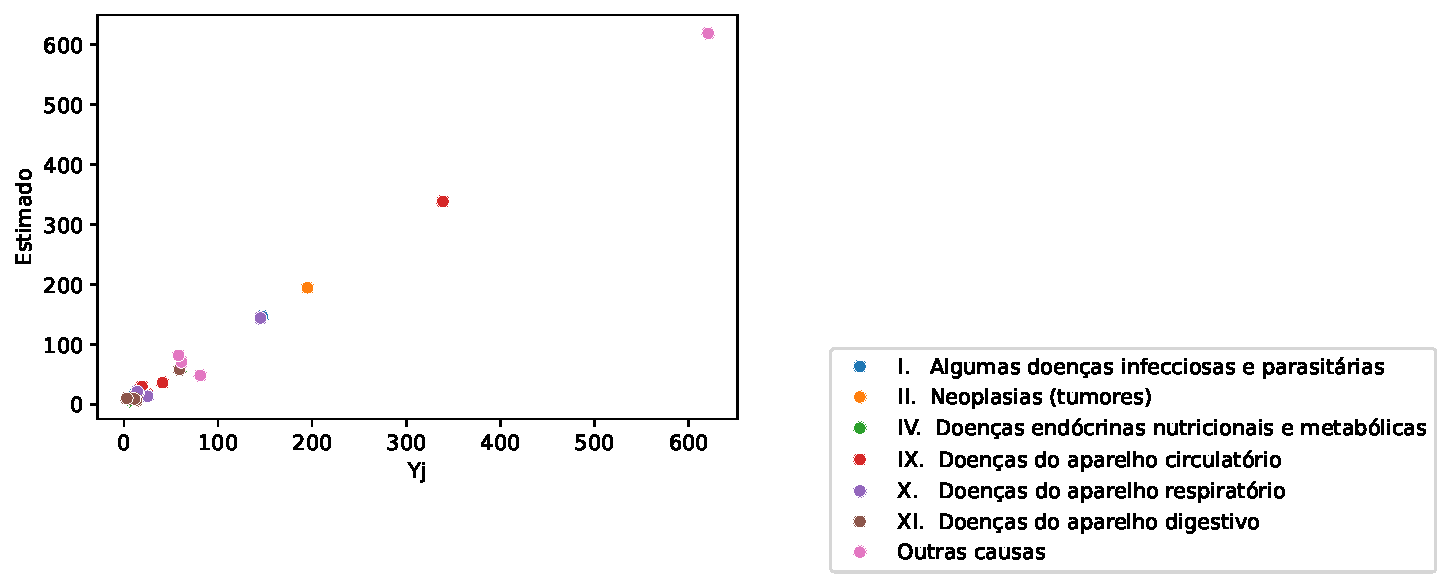
\includegraphics[keepaspectratio]{relatorio1_gabriel_pereira_files/figure-pdf/cell-16-output-1.pdf}}

}

\caption{Método Leadermann para o sexo masculino.}

\end{figure}%

\elandscape

\blandscape

A tabela abaixo apresenta os resultados obtidos para o sexo feminino.
Tanto a tabela quanto o gráfico dos valores estimados e observados
indicam que os valores estimados estão muito próximos dos valores reais,
exibindo um padrão semelhante ao observado para o sexo masculino.

\begin{longtable}[]{@{}lllll@{}}
\caption{Método de Leadermann para o sexo
feminino.}\label{T_17c09}\tabularnewline
\toprule\noalign{}
Causas & Região & Yj & Estimado & Bj \\
\midrule\noalign{}
\endfirsthead
\toprule\noalign{}
Causas & Região & Yj & Estimado & Bj \\
\midrule\noalign{}
\endhead
\bottomrule\noalign{}
\endlastfoot
I. Algumas doenças infecciosas e parasitárias & 14001 BOA VISTA & 87 &
86.425706 & 2.058797 \\
I. Algumas doenças infecciosas e parasitárias & 14002 NORDESTE DE
RORAIMA & 10 & 14.367821 & 2.058797 \\
I. Algumas doenças infecciosas e parasitárias & 14003 CARACARAI & 5 &
6.132634 & 2.058797 \\
I. Algumas doenças infecciosas e parasitárias & 14004 SUDESTE DE RORAIMA
& 9 & 4.073838 & 2.058797 \\
II. Neoplasias (tumores) & 14001 BOA VISTA & 181 & 180.457156 &
4.402005 \\
II. Neoplasias (tumores) & 14002 NORDESTE DE RORAIMA & 22 & 26.386964 &
4.402005 \\
II. Neoplasias (tumores) & 14003 CARACARAI & 9 & 8.778943 & 4.402005 \\
II. Neoplasias (tumores) & 14004 SUDESTE DE RORAIMA & 8 & 4.376937 &
4.402005 \\
IV. Doenças endócrinas nutricionais e metabólicas & 14001 BOA VISTA & 75
& 74.066545 & 1.747949 \\
IV. Doenças endócrinas nutricionais e metabólicas & 14002 NORDESTE DE
RORAIMA & 5 & 12.888332 & 1.747949 \\
IV. Doenças endócrinas nutricionais e metabólicas & 14003 CARACARAI & 8
& 5.896536 & 1.747949 \\
IV. Doenças endócrinas nutricionais e metabólicas & 14004 SUDESTE DE
RORAIMA & 9 & 4.148587 & 1.747949 \\
IX. Doenças do aparelho circulatório & 14001 BOA VISTA & 196 &
194.354603 & 4.608933 \\
IX. Doenças do aparelho circulatório & 14002 NORDESTE DE RORAIMA & 20 &
33.041933 & 4.608933 \\
IX. Doenças do aparelho circulatório & 14003 CARACARAI & 14 & 14.606199
& 4.608933 \\
IX. Doenças do aparelho circulatório & 14004 SUDESTE DE RORAIMA & 22 &
9.997265 & 4.608933 \\
X. Doenças do aparelho respiratório & 14001 BOA VISTA & 92 & 91.471741 &
2.148131 \\
X. Doenças do aparelho respiratório & 14002 NORDESTE DE RORAIMA & 12 &
16.287147 & 2.148131 \\
X. Doenças do aparelho respiratório & 14003 CARACARAI & 8 & 7.694622 &
2.148131 \\
X. Doenças do aparelho respiratório & 14004 SUDESTE DE RORAIMA & 9 &
5.546490 & 2.148131 \\
XI. Doenças do aparelho digestivo & 14001 BOA VISTA & 43 & 43.026436 &
1.071103 \\
XI. Doenças do aparelho digestivo & 14002 NORDESTE DE RORAIMA & 6 &
5.537830 & 1.071103 \\
XI. Doenças do aparelho digestivo & 14003 CARACARAI & 0 & 1.253418 &
1.071103 \\
XI. Doenças do aparelho digestivo & 14004 SUDESTE DE RORAIMA & 1 &
0.182315 & 1.071103 \\
Outras causas & 14001 BOA VISTA & 280 & 279.254330 & 6.666819 \\
Outras causas & 14002 NORDESTE DE RORAIMA & 39 & 45.915679 & 6.666819 \\
Outras causas & 14003 CARACARAI & 24 & 19.248405 & 6.666819 \\
Outras causas & 14004 SUDESTE DE RORAIMA & 14 & 12.581586 & 6.666819 \\
\end{longtable}

\begin{figure}[H]

{\centering \pandocbounded{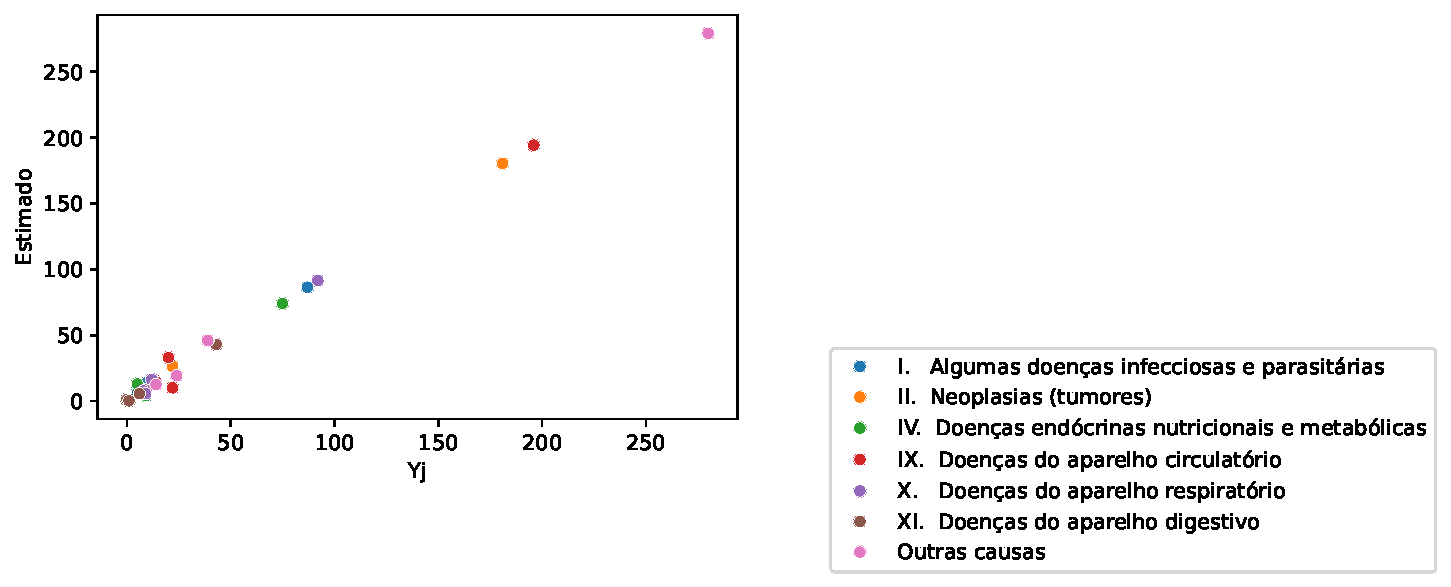
\includegraphics[keepaspectratio]{relatorio1_gabriel_pereira_files/figure-pdf/cell-19-output-1.pdf}}

}

\caption{Leadermann para o sexo feminino}

\end{figure}%

\elandscape

\chapter{Conclusão}\label{conclusuxe3o}

~~~Para a razão de sexo dos nascimentos no estado de Roraima, foi visto
que não apresenta víes de cobertura entre os sexos dos nascimentos. Em
relação aos métodos utilizados para estimação da cobertura de nascidos
vivos, o que apresentou melhores resultados foi o que utiliza os dados
do IBGE e SINASC, tendo obtido uma cobertura de 98,3\% para o ano de
2020.

\vspace{12pt}

Analisando-se os métodos utilizados para estimativa da cobertura de
óbitos, a maioria dos métodos não obtiveram boas estimativas,
principalmente o que fez uso da equação básica de crescimento
populacional, que acabou subestimando a estimativa de óbitos. O método
que obteve os melhores resultados foi o de Brass, tendo sido o melhore
para o ano de 2010, considerando-se o sexo masculino, embora ainda tenha
sido abaixo de uma estimativa significante, próxima de 68\%. Por último,
analisando-se o método de Leadermann para o sexo masculino e feminino,
os dois sexos apresentaram padrões bastante semelhantes para cada uma
das regiões.

\chapter*{\texorpdfstring{\centering Referências}{Referências}}\label{referuxeancias}

\markboth{Referências}{Referências}

\phantomsection\label{refs}
\begin{CSLReferences}{0}{1}
\bibitem[\citeproctext]{ref-quarto}
ALLAIRE, J.; DERVIEUX, C.
\textbf{\href{https://CRAN.R-project.org/package=quarto}{quarto: R
Interface to 'Quarto' Markdown Publishing System}}. {[}S.l.{]}:
{[}s.n.{]}, 2024.

\bibitem[\citeproctext]{ref-Hunter:2007}
HUNTER, J. D. \href{https://doi.org/10.1109/MCSE.2007.55}{Matplotlib: A
2D graphics environment}. \textbf{Computing in Science \& Engineering},
2007. v. 9, n. 3, p. 90--95.

\bibitem[\citeproctext]{ref-reback2020pandas}
TEAM, T. Pandas Development. \textbf{pandas-dev/pandas: Pandas}. Zenodo.
Disponível em:
\textless{}\url{https://doi.org/10.5281/zenodo.3509134}\textgreater.

\bibitem[\citeproctext]{ref-van1995python}
VAN ROSSUM, G.; DRAKE JR, F. L. \textbf{Python reference manual}.
{[}S.l.{]}: Centrum voor Wiskunde en Informatica Amsterdam, 1995.

\end{CSLReferences}




\end{document}
